\section{Dynamic Ranking Computation}
\label{sec-incAlg}

Scholarly articles are dynamic, and it is impractical to recompute ranking from scratch once they get updated. In this section, we present an incremental algorithm for our ranking model \ensemblerank.


\subsection{Incremental Algorithm Framework}
\label{subsec-inc-alg}




Our incremental algorithm \incensemble incrementally computes the popularity and prestige of scholarly articles.
We consider an update $\Delta$ = $\Delta V\cup\Delta E$ is added to a   (citation or venue) graph $G(V, E)$,
and the resulting graph is denoted as $G^+(V\cup\Delta V, E\cup\Delta E)$, where
$\Delta V\cap V = \emptyset$ is a set of nodes, and $\Delta E$ is a set of directed edges on $\Delta V$ and from $\Delta V$ to $V$ only, as article citations obey a natural temporal order, \ie an article only cites those published earlier, and it is really rare for the mutual citation of two articles published in the same time.


\stitle{Incremental popularity computation}.
The popularity of venues and authors is computed along the same lines as their batch counterparts of algorithm \batensemble,
as almost all venues and authors are affected  by the definitions of the popularity of venues and authors.


As the popularity of articles is defined as the freshness sum of all their citations, it is convenient to maintain. Consider an updated citation graph $G^{c,+}(V^c\cup\Delta V^c, E\cup\Delta E^c)$ of $G^c(V^c, E^c)$,  the updated popularity $pop_{c}^+(v)$ can be easily computed as:
\begin{small}
\begin{equation}\label{eq-inc-pop}
pop_c^+(v) = pop_c(v) {e^{\sigma (T^+_0-T_0)}} + \sum_{(u,v)\in \Delta E^c} {e^{\sigma (T^+_0-T_u)}}.
\end{equation}
\end{small}
\noindent
Where $pop_c(v)$ (resp. $pop_c^+(v)$) is the popularity of node $v$ on $G^c$ (resp. $G^{c,+}$), and
 $T_0$ (resp. $T^+_0$) is the current time in $G^c$ (resp. $G^{c,+}$).
%
By Eq.~(\ref{eq-inc-pop}), it is easy to see that it takes $O($ $|V^c|+|\Delta V^c|+|\Delta E^c|)$ time to update the popularity of articles.
%This further shows that Eq.~(\ref{eq-inc-pop}) is a desired solution for popularity maintenance.



\stitle{Incremental prestige computation}.
The prestige of authors is computed along the same lines as their batch counterparts of algorithm \batensemble,
as almost all authors are affected  by the definition of the prestige of authors.
%
For the prestige of articles and venues, we propose an incremental algorithm to maintain their prestige.



%We first present the incremental  prestige computation. Again, it differs for the prestige of articles and venues in a specific year and the one of authors. We finally present the complete incremental algorithm \incensemble, which is similar to the batch algorithm \batensemble, except that (1) it uses algorithm \inctwprscc to incrementally compute the prestige of articles and venues, and (2) it incrementally computes the popularity of articles based on Eq.~(\ref{eq-inc-pop}).




\subsection{Incremental TWPageRank Computation}
\label{subsec-incTWPageRank-computation}

%\subsubsection{Prestige of articles and venues in a specific year}
%\label{subsubsec-incprs-CV}
%\subsubtitle{Prestige of articles and venues in a specific year}.
%We expand $M$ and $PR$ to the same sizes as $M^+$ and $PR^+$, respectively, by filling zeros, and let $\Delta M=M^+ - M$ and $\Delta PR = PR^+ - PR$.



%%%%%%%%%%%%%%%%%%%%%Algorithm
\begin{figure}[tb!]
%\vspace{2ex}
\begin{center}
{\small
\begin{minipage}{3.36in}
\myhrule \vspace{-1.5ex}
\mat{0ex}{
%%%%%%%%%%%%%%%%%%%
{\sl Input:\/} \= An update $\Delta$ = $\Delta V\cup\Delta E$, TWPageRank vector $PR$ of $G$,  and the   \\
\hspace{6ex} topological order $O$ of the block-wise graph $G'(V',E')$.\\
{\sl Output:\/} TWPageRank vector $PR^+$ of the updated graph $G^+$. \\
\bcc \hspace{1.5ex}\=  $G_C'$ := the block-wise graph of $G_C$; \\
%\ \  $E_{CB}'$ := edges from $G_C'$ to $G'$\\
\icc\> $\Delta O$ := topological order of $G_C'$; \ \ $O^+$ := $\Delta O/O$; \\
\icc\> label all SCCs of $G$ with outgoing edges having weight changes as $B$, \\ \hspace{2.5ex} all remailing SCCs of $G$ as $A$ and all SCCs of $G_C$ as $C$;\\
\icc\>  \For each node $v'$ following $O^+$ \Do\\
\icc\>\hspace{2.5ex}\= $scc$ := the corresponding SCC of $v'$; \\
%\icc\>\>\If impact weight of $(v,w)$ is changed where $v\in scc$ \Then \\
%\icc\>\>\hspace{3ex}\= label $scc$ as $B$;\\
%\icc\>\>\> label SCC $w'$ as $B$ such that $(v',w')\in E'$; \\
\icc\>\> \If $scc$ is labeled as $C$ \Then \\
\icc\>\>\hspace{3ex}\= update $PR^+(v)$ where $v\in scc$ following algorithm~\twprscc; \\
\icc\>\>\> label SCC $w'\in G'$ as $B$ such that $w'$ is reachable from $w$;\\
\icc\>\> \Else \If $scc$ is labeled as $B$ \Then \\
\icc\>\>\> update $PR^+(v)$ where $v\in scc$ with Eq.~(\ref{eq-inc-prscc}) until the sum of \\ \hspace{8ex} TWPageRank score changes is less than $\epsilon\cdot |scc|/|V^+|$; \\
\icc\>\>\> label SCC $w'$ as $B$ such that $(v',w')\in E'$;\\
\icc\>\> \Else $PR^+(v)$:=$PR(v)\cdot {n}/{n^+}$ where $v\in scc$; \\
\icc\> \Return $PR^+$.
}
\vspace{-2.5ex} \myhrule
\end{minipage}
}
\end{center}
\vspace{-3ex}
\caption{\small Algorithm~\inctwprscc for incremental TWPageRank} \label{alg-inctwprscc}
\vspace{-3ex}
\end{figure}
%%%%%%%%%%%%Algorithm

Consider a citation or venue graph $G(V, E)$, its TWPageRank vector $PR$ and the topological order $O$ of its block-wise graph. Given an update $\Delta$ = $\Delta V\cup\Delta E$ to $G$, the incremental prestige computation for articles and venues in a specific year is to compute the TWPageRank vector $PR^+$ on the updated graph $G^+(V\cup\Delta V, E\cup\Delta E)$.


\stitle{Auxiliary data structure maintenance}.
Two auxiliary data structures in the batch algorithm~\twprscc need to be maintained : (a) the block-wise graph,  a mapping that, given a node of graph $G$, returns the index of the \scc to which it belongs, and (b) the topological order of the nodes in the block-wise graph.
%
Observe that these auxiliary data structures can be easily maintained as follows.

%the idea is to divide $G$ into affected and unaffected areas such that TWPageRank scores of nodes in affected and unaffected areas are updated accordingly.


\sstab(1) The block-wise graph of $G^+$ needs to be computed, whose \sccs consist of the \sccs in $G$ and \sccs in the induced subgraph $G^+[\Delta V]$, as  the edges $\Delta E$ are  on $\Delta V$ and from $\Delta V$  to $V$ only. Hence, only those new \sccs in $G^+[\Delta V]$ need to be computed.

\sstab(2) The the topological order $O^+=\Delta O/O$, where $\Delta O$ is the topological order of the block-wise graph of $G^+[\Delta V]$. Hence, only $\Delta O$ needs to be computed. One can easily verify the following.


\begin{prop} \label{lemma-inc-topo}
 $O^+=\Delta O/O$ is indeed a valid topological order of the block-wise graph of $G^+$.
\end{prop}

\eat{%%%%%%%%%%%
\begin{proof}
Let $E'_c$ denote the set of cross edges from $V'_\Delta$ to $V'$.
It suffices to show that for each $(u,v)\in E'\cup E'_\Delta \cup E'_c$, $u$ comes before $v$ in $O^+$,
which obviously holds (1) for  $E'\cup E'_\Delta$ as $O$ and $\Delta O$ are topological orders of $G'$ and $G'_\Delta$, respectively, and (2) for $E_{c}'$ as nodes in $G'_\Delta$ come before nodes in $G'$.
\end{proof}
}%%%%%%%%%%%%


%%% affected/unaffected division
\stitle{Analyses of affected and unaffected areas}.
The TWPageRank vector $PR$ of graph $G$ is mainly affected in two ways.



\sstab(1) Let $V_{B,1}\subseteq V$ be the set of nodes reachable from the newly added nodes $\Delta V$ in $G^+$, $V_{B,2}\subseteq V$ be the set of nodes with outgoing edges having weight changes, and $V_{B,3}\subseteq V$ be the set of nodes reachable from  $V_{B,2}$.
%
Then $V_B=V_{B,1}\cup V_{B,2}\cup V_{B,3}$ is obviously the set of nodes in $G$ affected by the update $\Delta$.
%
As a result, TWPageRank scores on $V_B$ are recomputed with iterations.
%using the existing TWPageRank vector scaled with constant ${n}/{n^+}$.
%
\begin{small}
\begin{equation}\label{eq-inc-prscc}
\begin{split}
PR^+(v) \ = \ &  d \sum_{(u,v)\in E^+_i} M^+_{u,v} PR^+(u) + d \sum_{(u,v)\in E^+_a} M^+_{u,v} PR^+(u)  \\
 + \frac{n}{n^+} \Big( PR(v) &  - d \sum_{(u,v)\in E_i} M_{u,v} PR(u) - d\sum_{(u,v)\in E_a} M_{u,v} PR(u)\Big).
\end{split}
\end{equation}
\vspace{-2ex}
\end{small}

\sstab(2) Let $V_A = V\setminus V_B$. Since $V_A$ are not reachable from newly added or affected nodes, $V_A$ is essentially not affected by the update $\Delta$. And TWPageRank scores on $V_A$ can be simply adjusted by scaling existing results with constant ${n}/{n^+}$.

Let $G_A=(V_A,E_A)$, $G_B=(V_B,E_B)$ and $G_C=(V_C,E_C)$, respectively, and
let $E_{AB}$ and $E_{CB}$  be the sets of edges from $G_A$ to $G_B$ and from $G_C$ to $G_B$, respectively.
In this way, graph $G^+$ is divided into subgraphs $\{G_A$, $G_B$, $G_C\}$ and edge sets $\{E_{AB}, E_{CB}\}$.
%
We then have $G_C$ = $G^+[\Delta V]$, $\Delta E$ = $E_C\cup E_{CB}$, $V$ = $V_A\cup V_B$ and $E$ = $E_A\cup E_B\cup E_{AB}$.

\marked{
Observe that $M_{u,v}=M^+_{u,v}$ and $PR^+(u)={n}/{n^+}\cdot PR(u)$ for nodes $u$ such that $(u,v)\in E_{AB}$. Therefore, the process on $V_B$ in Eq.~(\ref{eq-inc-prscc}) can skip the edges in $E_{AB}$. Moreover, we use ${n}/{n^+}\cdot PR$ as the initial iteration vector. Both of them can speed up the computation.
}

\stitle{Incremental algorithm \inctwprscc}. We now present our algorithm for incremental TWPageRank  computation, shown in Fig.~\ref{alg-inctwprscc}.


It takes as input an update $\Delta$ and the previous results on the original graph $G(V, E)$, and returns the TWPageRank vector of the updated graph $G^+$. It first incrementally computes the topological order $O^+$
%by concatenating the topological orders of $G_C'$ and $G'$
(lines 1--2). %Note that $G_C'$ is the same to $G'_\Delta$.
%
After that, it labels the newly added \sccs with $C$ and existing \sccs with $A$ or $B$, depending on whether the existing \sccs have outgoing edges with weight changes (line 3).
%
It then updates the TWPageRank scores of nodes in each \scc following $O^+$ according to the labels (lines 4--12) and finally returns the TWPageRank vector (line 13).
%
%More specifically, the scores of nodes in SCCs labeled as $C$ and $B$ are updated the same to Algorithm~\twprscc, while the scores of nodes in SCCs labeled as $A$ are simply scaled.
%
%It is also easy to verify that nodes in SCCs labeled as $A$, $B$ and $V$ corresponding to $V_A$, $V_B$ and $V_C$.

\eat{
\begin{figure}[tb!]
\centering
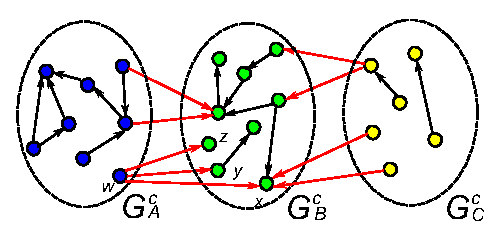
\includegraphics[scale=0.6]{fig/General_framework_peak_ABC.eps}
\vspace{-3ex}
\caption{\small An example of affected and unaffected areas}
\label{fig-inc-division}
\vspace{-3ex}
\end{figure}
}

\begin{figure}[tb!]
\centering
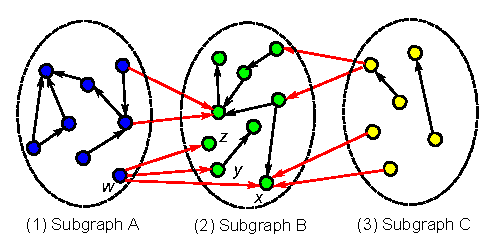
\includegraphics[scale=0.6]{fig/General_framework_peak.eps}
\vspace{-3.5ex}
\caption{\small An example of incremental TWPageRank computation}
\label{fig-inc-division}
\vspace{-4ex}
\end{figure}

\eat{
\begin{example} \label{eg-layer-dag}
Figure~\ref{fig-inc-division} illustrates an example of affected and unaffected areas, in which subgraphs $G_A$, $G_B$ and $G_C$ are associated with node sets $V_A$, $V_B$ and $\Delta V$, respectively. Here the citation peak time of node $x$ is changed, which leads to the changes of the normalized weights of edges $(w,x)$, $(w,y)$ and $(w,z)$.
\end{example}
}
\begin{example} \label{eg-layer-dag}
Figure~\ref{fig-inc-division} illustrates an example of incremental TWPageRank computation. Consider an update $\Delta$ on the original graph $G$.
%
It is obvious that the update $\Delta$ has on impacts on the SCCs of $G$, and $O^+$ defined earlier is a valid topological order of $G^+{'}$.
%
The original graph $G$ is then divided into affected and unaffected areas, in which subgraphs $G_A$, $G_B$ and $G_C$ are associated with node sets $V_A$, $V_B$ and $\Delta V$, respectively. Here the citation peak time of node $x$ is changed, and, hence, node $y$ as well as all nodes reachable from $y$ are included in $G_B$.
%
When updating the TWPageRank scores, following $O^+$, scores of nodes in $G_C$, $G_B$ and $G_A$ are computed by iterations from scratch, by iterations using existing TWPageRank vector and by scaling, respectively.
\end{example}

\begin{theorem}
\label{lemma-subgraphA}
The TWPageRank vector $PR^+$ returned by~\inctwprscc converges such that $||PR^+-PR^{*}||_1 < \epsilon$, where $PR^{*}$ is the convergent TWPageRank vector.
\end{theorem}

\begin{proofSketch}
Assume a topological order $v_1'/\dots/v_{l}'$ of graph $G^+{'}$ where $l=|O^+|$. It suffices to prove the sum of change of $PR^+(v)$ where $v\in scc_k$ is no more than $|scc_k|\cdot\epsilon/n^+$ for $scc_k$ corresponding to $v_k'$ ($k\in [1,l]$) by induction.
%The conclusion follows combining Lemma~\ref{prop-prscc}
(see \cite{SARank-full} for details).
\end{proofSketch}


The main result here is stated as follows.


\begin{prop} \label{lemma-inc-citation-comp}
Given an update $\Delta$ = $\Delta V\cup\Delta E$ of graph $G(V,E)$, and the TWPageRank vector and topological order of the  the
block-wise graph of $G$, algorithm \inctwprscc runs in $O(|V\cup \Delta V|+|E_B\cup E_C\cup E_{CB}|+t^+|E_{B,i}\cup E_{C,i}|)$ time.
\end{prop}

\begin{proof}
Observe the following. (1) A topological order of $G_C$ can be computed in $O(|V_C|+|E_C|+|E_{CB}|)$ time.
(2) Updating the TWPageRank scores of nodes in subgraphs $G_B$ and $G_C$ costs $O(|V_B\cup V_C|+|E_{B,a}\cup E_{C,a}\cup E_{CB}|)+t^+|E_{B,i}\cup E_{C,i}|)$ time. Finally, (3) Updating the scores of nodes in $G_A$ costs $O(|V_A|)$ time.
\end{proof}

%Note that the incremental algorithm reduces the complexity of updating subgraph $A$ from $O(|E^c_A|)$ to $O(|V^c_A|)$. It is more effective when only a small number of articles are updates, resulting in $|V^c_A|>>|V^c_B|+|V^c_C|$ and updating subgraph $A$ occupies most of the computation.

By Propositions~\ref{prop-converg} \& \ref{lemma-inc-topo} and Theorem \ref{lemma-subgraphA}, one can easily verify the correctness of algorithm \inctwprscc.
%
Note that  a) algorithm \inctwprscc computes \sccs and derives the topological order based  on $\Delta$ only, instead of $G^{+}$,
b) it skips edges in $E_A\cup E_{AB}$ when updating the scores of nodes in $G_A$ and $G_B$, and
c) the number $t^+$ is very likely smaller than the number $t$ of \twprscc when updating scores of nodes in $V_B$.
%
All these make \inctwprscc faster than \twprscc even though they have very similar time complexity. 
%, as will also been shown by the experimental study,

\marked{
\stitle{Time \& space complexity analyses of the complete algorithm}.
By the analyses above, the time complexity of \incensemble is the same as \batensemble, except that \incensemble saves $O(|E^c_A\cup E^c_{AB}|)$ and $O(|E^v_A\cup E^v_{AB}|)$ time on the updated citation graphs and venue graphs when updating scores. And its space complexity is also the same as \batensemble, except that it uses $(|V^c\cup\Delta V^c|+|V^v\cup\Delta V^v|)$ extra space to store the affected/unaffected areas and $|E^c\cup \Delta E^c|+|E^v\cup \Delta E^v|$ extra space to store original edge weights.
}

\marked{
Indeed, algorithm \incensemble is typically faster than \batensemble as follows.
(a) It saves $O(|V^c|+|E^c|)$ and $O(|V^v|+|E^v|)$ time when maintaining \sccs and the topological order based on $G^c_C$ and $G^v_C$;
(b) It saves $O(|E^c_A \cup E^c_{AB}|)$ and $O(|E^v_A \cup E^v_{AB}|)$ time when updating scores on $V^c$ and $V^v$;
(c) It saves $O(|E^c|)$ time when computing popularity of articles;
And, finally, (d) It is likely to compute TWPageRank scores on $V^c_B$ and $V^v_B$ with less iterations.
%
According to our statistics on citation and venue graphs in Table 2, $|V_A\cup V_B|$ (\ie $|V|$) and $|E_A\cup E_{AB}\cup E_B|$ (\ie $|E|$) are more than 89\% of $|V^+|$ and $|E^+|$ on all graphs, respectively, and $E_A\cup E_{AB}$ accounts for 28\% of total edges on all citation graphs.
}
%
%

\eat{
Indeed, algorithm \incensemble is typically faster than \batensemble in practice as follows.
(1) It computes \sccs and derives the topological order on $G^c_C$ and $G^v_C$ in $O(|\Delta V^c|+|\Delta E^c|)$ %(comparatively, $O(|V^c\cup\Delta V^c|+|E^c\cup \Delta E^c|)$)
and $O(|\Delta V^v|+|\Delta E^v|)$ %(comparatively, $O(|V^v\cup \Delta V^v|+|E^v\cup \Delta E^v|)$)
time;
(2) It saves $O(E^c_A \cup E^c_{AB})$ and $O(E^v_A \cup E^v_{AB})$ time when updating scores on $V^c$ and $V^v$;
(3) It computes popularity of articles in $O(|V^c\cup\Delta V^c|+|\Delta E^c|)$ %(comparatively, $O(|V^c\cup\Delta V^c|+|E^c\cup \Delta E^c|)$)
time;
And, finally, (4) It is likely to update TWPageRank scores on $V^c_B$ and $V^v_B$ with less iterations.
}
%The efficiency improvement is achieved by using $(|V^c\cup\Delta V^c|+|V^v\cup\Delta V^v|)$ extra space to store the affected and unaffected areas.






%%%%%%%%%%%%%%%%%%%%%%%%%%%%%%%%%%%%%%%%%%%%%%%%%%
\begin{table}[tb!]
%\vspace{-2ex}
\begin{center}
\begin{small}
\vspace{1ex}
\eat{
\begin{tabular}{|c|c c c|c c c|}
\hline
{\bf Graphs} & $|V_A|$ & $|V_B|$ & $|V_C|$ & $|E_A\cup E_{AB}|$ & $|E_B|$ & $|E_C\cup E_{CB}|$ \\
\hline \hline
% citation graphs
\aan & $46.9\%$ & $47.3\%$ & $5.8\%$ & $28.8\%$ & $60.5\%$ & $10.7\%$ \\
\aminer & $81.4\%$ & $10.7\%$ & $7.8\%$ & $71.2\%$ & $25.1\%$ & $3.7\%$ \\
\magdata & $69.5\%$ & $25.9\%$ & $4.5\%$ & $28.4\%$ & $64.5\%$ & $7.1\%$ \\ \hline
% venue graphs
\aan & $2.1\%$ & $92.0\%$ & $5.8\%$ & $1.0\%$ & $88.8\%$ & $10.2\%$ \\
\aminer & $45.8\%$ & $47.7\%$ & $6.4\%$ & $3.5\%$ & $95.4\%$ & $1.1\%$ \\
\magdata & $12.4\%$ & $84.6\%$ & $3.0\%$ & $0.1\%$ & $92.6\%$ & $7.3\%$ \\ \hline
}
%\eat{
\begin{tabular}{|c|c|c|}
\hline
{\bf Graphs} & $|V_A|$\hspace{2ex}$|V_B|$\hspace{3ex}$|V_C|$ & $|E_A|$\hspace{2ex}$|E_{AB}|$\hspace{2ex}$|E_B|$\hspace{2ex}$|E_{CB}|$\hspace{2ex}$|E_C|$ \\
\hline \hline
% citation graphs
\aan & $46.9\%$ \hspace{1ex} $47.3\%$ \hspace{1ex} $5.8\%$ & \ $2.9\%$ \hspace{1ex} $25.9\%$ \hspace{1ex} $60.5\%$ \hspace{1ex} $10.4\%$ \hspace{1ex} $0.3\%$ \\
\aminer & $81.4\%$ \hspace{1ex} $10.7\%$ \hspace{1ex} $7.8\%$ & $18.0\%$ \hspace{1ex} $53.2\%$ \hspace{1ex} $25.1\%$ \hspace{1ex} \ $2.3\%$ \hspace{1ex} $1.4\%$ \\
\magdata & $69.5\%$ \hspace{1ex} $25.9\%$ \hspace{1ex} $4.5\%$ & \ $1.0\%$ \hspace{1ex} $27.4\%$ \hspace{1ex} $64.5\%$ \hspace{1ex} \ $7.0\%$ \hspace{1ex} $0.1\%$ \\ \hline
% venue graphs
\aan & \ $2.1\%$ \hspace{1ex} $92.0\%$ \hspace{1ex} $5.8\%$ & \ $1.0\%$ \hspace{1ex} \ $1.0\%$ \hspace{1ex} $88.8\%$ \hspace{1ex} $10.0\%$ \hspace{1ex} $0.2\%$ \\
\aminer & $45.8\%$ \hspace{1ex} $47.7\%$ \hspace{1ex} $6.4\%$ & \ $0.0\%$ \hspace{1ex} \ $3.2\%$ \hspace{1ex} $95.4\%$ \hspace{1ex} \ $1.0\%$ \hspace{1ex} $0.1\%$ \\
\magdata & $12.4\%$ \hspace{1ex} $84.6\%$ \hspace{1ex} $3.0\%$ & \ $0.0\%$ \hspace{1ex} \ $0.1\%$ \hspace{1ex} $92.6\%$ \hspace{1ex} \ $7.1\%$ \hspace{1ex} $0.1\%$ \\ \hline
%}
\end{tabular}
\end{small}
\end{center}
\caption{\small Statistics of affected/unaffected areas on citation graphs (rows 2--4) and venue graphs (rows 5--7) given a yearly update, \ie articles of 2011 on \aan and of 2015 on \aminer and \magdata, respectively.}
\label{tab-inc}
\vspace{-6ex}
\end{table}
%%%%%%%%%%%%%%%%%%%



\eat{  %%%%%%%%%%%%%%%%%%%%%%%%%%%%% ensemble version
\subsection{Incremental Citation Ensemble}
\label{subsec-inc-citation}

We first present the incremental computation of prestige and popularity for the citation ensemble.
Consider an update $\Delta^c$ = $\Delta V^c\cup\Delta E^c$ added to citation graph $G^c(V^c, E^c)$,
and the resulting citation graph is $G^{c,+}(V^c\cup\Delta V^c, E^c\cup\Delta E^c)$, where
 $\Delta V^c$ is a set of nodes with $\Delta V^c\cap V^c = \emptyset$, and $\Delta E^c$ is a set of directed edges on $\Delta V^c$ and from $\Delta V^c$ to $V^c$ only, by the temporal order of citations.



\eat{The main result here is stated as follows.

\begin{theorem}
\label{thm-inc-citation}
Given a citation graph $G^c$ and a update citation graph $\Delta G^c$, incremental TWPageRank and incremental popularity computation on $G^c_+$ can be done in $O(|V^c_+|+|E^c_B|+|E^c_C|+|E^c_{AB}|+|E^c_{CB}|)$ and $O(|V^c_+|+|\Delta E^c|)$, respectively.
\end{theorem}

As will be seen shortly, $E^c_B$, $E^c_C$, $E^c_{AB}$ and $E^c_{CB}$ are derived by dividing the base citation graph into {\em affected and unaffected areas}, and $|E^c_B|+|E^c_C|+|E^c_{AB}|+|E^c_{CB}|=|E^c_+|-|E^c_A|<|E^c|$ in practice. By comparison, the complexities of  the batch algorithm \batensemble are $O(|V^c_+|+|E^c_+|)$ and $O(|E^c_+|)$, respectively.

We prove Theorem~\ref{thm-inc-citation} by proving algorithms for incremental TWPageRank and incremental popularity computation with desired properties, respectively.
}


\begin{figure}[tb!]
\centering
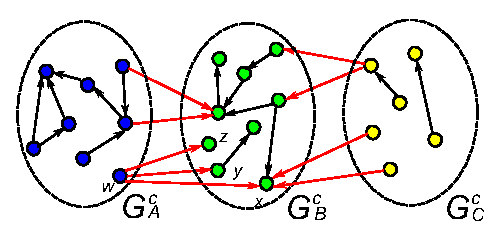
\includegraphics[scale=0.6]{fig/General_framework_peak_ABC.eps}
\vspace{-2ex}
\caption{\small An example of affected and unaffected areas}
\label{fig-inc-division}
\vspace{-3ex}
\end{figure}

\subsubsection{Incremental Prestige Computation}

%Give graph $G=(V,E)$, the TW PageRank score $PR(v)$ only depends on scores $PR(u)$ such that $(u,v)\in E$, as indicated by Eq.~(\ref{eq-twpr}). In other words, each node $u$ has a limited area, instead of the entire $G$, such that the PageRank scores of nodes within the area are affected by $PR(u)$.
%This motivates us to incrementally compute TWPageRank scores by dividing the existing graph into affected and unaffected areas in terms of the update citation graph $\Delta G^c$.
We first present how to incrementally compute the prestige of the citation ensemble, \ie the TWPageRank vector on the updated citation graph $G^{c,+}$,
given an update $\Delta^c$ = $\Delta V^c\cup\Delta E^c$ and the TWPageRank vector on the original citation graph $G^{c}$.

%Observe that the update $\Delta$ to citation $G^c$ has certain impacts on part of the base citation graph $G^c$, instead of the entire $G^c$. Hence, TWPageRank is computed incrementally by dividing $G^c$ into affected and unaffected areas and using different incremental updating strategies for nodes in affected and unaffected areas, respectively.


%%% affected/unaffected division
\stitle{Affected and unaffected areas}.
The TWPageRank vector of the original citation graph $G^{c}$ is mainly affected in two ways.



\sstab(1) Let $V^c_{B,1}\subseteq V^c$ be the set of nodes reachable from the newly added nodes $\Delta V^c$ in $G^{c,+}$, $V^c_{B,2}\subseteq V^c$ be the set of nodes with incoming edges having weight changes, and $V^c_{B,3}\subseteq V^c$ be the set of nodes reachable from  $V^c_{B,2}$.

Then $V^c_B=V^c_{B,1}\cup V^c_{B,2}\cup V^c_{B,3}$ is obviously the set of nodes in $G^{c}$ affected by the update $\Delta^c$.


\sstab(2) Let $V^c_A = V^c\setminus V^c_B$. As the TWPageRank scores on $V^c_A$ can be simply adjusted by scaling in terms of  Lemma~\ref{lemma-subgraphA} (to be seen shortly), $V^c_A$ is essentially not affected by the update $\Delta^c$.

Let $G^c_A=(V^c_A,E^c_A)$, $G^c_B=(V^c_B,E^c_B)$ and $G^c_C=(V^c_C,E^c_C)$, respectively;
Let $E^c_{AB}$ be the set of edges from $G^c_A$ to $G^c_B$, and $E^c_{CB}$ be the set of edges from $G^c_C$ to $G^c_B$.
%
Then we have $V^c_C$ = $\Delta V^c$, $E^c_C\cup E^c_{CB}$ = $\Delta E^c$, $V^c$ = $V^c_A\cup V^c_B$, and $E^c$ = $E^c_A\cup E^c_B\cup E^c_{AB}$.

In this way, the updated citation graph $G^{c,+}$ is partitioned into (a) subgraphs $\{G^c_A$, $G^c_B$, $G^c_C\}$ and (b) edge sets $\{E^c_{AB}$, $E^c_{CB}\}$.







\begin{example} \label{eg-layer-dag}
Figure~\ref{fig-inc-division} illustrates an example of affected and unaffected areas, in which subgraphs $G^c_A$, $G^c_B$ and $G^c_C$ are associated with node sets $V^c_A$, $V^c_B$ and $\Delta V^c$, respectively. Here the citation peak time of node $x$ is changed, which leads to the changes of the normalized weights of edges $(w,x)$, $(w,y)$ and $(w,z)$.
\end{example}

 We now present the incremental update rule.

%Intuitively, PageRank scores of nodes in $G_B$ are directly affected by $G_C$ and need to be recomputed, while PageRank scores of nodes in $G_A$ are only scaled due to the increment of $n$.
%We use notations without/with label  to denote corresponding values before/after adding subgraph $C$, and notations with label $\Delta$ to denote changes of values after adding subgraph $C$, \eg $\Delta PR(v)=PR^+(v)-PR(v)$.
%The base graph $G=(V, E)$, update graph $\Delta G=(\Delta V, \Delta E)$ and new graph $G^+=(V^+,E^+)$ are given by $G_A+G_B+E_{AB}$, $G_C+E_{CB}$ and $G+\Delta G$, respectively.

\stitle{Incremental update rule}. Here notations without/with superscript `$+$' are defined on $G^c$ and $G^{c,+}$, respectively.
We expand $M$ and $PR$ to the same sizes as $M^+$ and $PR^+$, respectively, by filling zeros, and let $\Delta M=M^+ - M$ and $\Delta PR = PR^+ - PR$.

The TWPageRank vector $PR^+$ on the original part of $G^{c,+}$, \ie $G^c$,  is incrementally updated as follows.
\begin{small}
\begin{equation}\label{eq-inc-prdag}
\begin{split}
PR^+(v) = &\frac{1-d}{n^+}+d \sum_{(u,v)} (M_{u,v}+\Delta M_{u,v}) (PR(u) + \Delta PR(u)) \\
  % = & \frac{n}{n^+} (\frac{1-d}{n}+d \sum_{(u,v)\in E} M_{u,v} PR(u)) \\
 = &\frac{n}{n^+} PR(v) + d \sum_{(u,v)} M_{u,v} (\frac{n^+-n}{n^+} PR(u) + \Delta PR(u)) \\
   &+ d \sum_{(u,v)} \Delta M_{u,v} PR^+(u).
\end{split}
\end{equation}
\end{small}

\vspace{-1ex}
\noindent
Here $(u,v)\in E^c\cup\Delta E^c$, and $M_{u,v}=0$ when $(u,v) \in \Delta E^c$.





%%%%%%%%%%%%%%%%%%%%%Algorithm
\begin{figure}[tb!]
%\vspace{2ex}
\begin{center}
{\small
\begin{minipage}{3.36in}
\myhrule \vspace{-2ex}
\mat{0ex}{
%%%%%%%%%%%%%%%%%%%
{\sl Input:\/} \= An update $\Delta^c$ = $\Delta V^c\cup\Delta E^c$, TWPageRank vector $PR$,  matrix $M$, \\
\hspace{6ex}  and the topological order $O$ of the original citation graph $G^c$.\\
{\sl Output:\/} TWPageRank vector $PR^+$ of the updated citation graph $G^{c,+}$. \\
\bcc \hspace{1.5ex}\=  $\Delta O$ := topological order of $G^c_C$; \ \ $O^+$ := $\Delta O/O$; \\
\icc\> label all nodes of $G^c$ as $A$ and all nodes of $G^c_C$ as $C$;\\
\icc\>  \For each node $v$ following $O^+$ \Do\\
\icc\>\hspace{2.5ex}\= \If $v$ is labeled as $C$ \Then \\
\icc\>\> \hspace{3ex}\= update $PR^+(v)$ using Eq.~(\ref{eq-twpr}); \\
\icc\>\>\> label node $w$ as $B$ such that $w\in V^c$ and $(v,w)\in \Delta E^c$;\\
\icc\>\> \Else \If $v$ is labeled as $B$ \Then \\
\icc\>\>\> update $PR^+(v)$ using Eq.~(\ref{eq-inc-prdag}); \\
\icc\>\>\> label node $w$ as $B$ such that $(v,w)\in E^c$;\\
\icc\>\> \Else $PR^+(v)$:=$PR(v)\cdot {n}/{n^+}$; \\
\icc\>\>\> \If $W(v)$ is changed \Then \\
\icc\>\>\>\hspace{2ex} label node $w$ as $B$ such that $(v,w)\in E^c$; \\
\icc\> \Return $PR^+$.
}
\vspace{-3ex} \myhrule
\end{minipage}
}
\end{center}
\vspace{-3ex}
\caption{\small Algorithm \inctwprdag} \label{alg-inctwprdag}
\vspace{-3ex}
\end{figure}
%%%%%%%%%%%%Algorithm

\stitle{Algorithm \inctwprdag}. We now present our incremental algorithm for the prestige computation, shown in Fig.~\ref{alg-inctwprdag}.

It takes as input an update $\Delta^c$ and the previous results on the original citation graph $G^c(V^c,E^c)$, and returns the TWPageRank vector of the updated citation graph $G^{c,+}$. It first derives a topological order $\Delta O$ of $G^c_C$, and concatenates $\Delta O$ with $O$ (line 1). After that, it labels the newly added nodes with $C$ and existing nodes with $A$ (line 2). It then updates the TWPageRank score of each node following $O^+$ (lines 3--12). More specifically, the scores of nodes labeled as $C$ and $B$ are updated according to Eq.~(\ref{eq-twpr}) and Eq.~(\ref{eq-inc-prdag}), respectively, while the scores of nodes labeled as $A$ are simply scaled. It finally returns the TWPageRank vector (line 13).

%%% algorithmic correctness
%We now show that \inctwprdag is indeed the desired algorithm for incremental TWPageRank on citation graphs.



\begin{lemma} \label{lemma-inc-topo}
$O^+$ is indeed a valid topological order of $G^{c,+}$.
\end{lemma}

\begin{proof}
It suffices to show that for each $(u,v)\in E^c\cup E^c_{C}\cup E^c_{CB}$, $u$ comes before $v$ in $O^+$,
which obviously holds (1) for  $E^c\cup E^c_{C}$ as $O$ and $\Delta O$ are topological orders of $G^c$ and $G^c_C$, respectively, and (2) for $E^c_{CB}$ as nodes in $G^c_C$ come before nodes in $G^c_B$.
%It obviously holds for each $(u,v)\in E^c+E^c_{C}$ since $O$ and $\Delta O$ are valid topological orderings of $G^c$ and $\Delta G^c$, respectively.
%It also holds for each $(u,v)\in E^c_{CB}$ since nodes in subgraph $C$ come before nodes in Subgraph $B$ in $O_+$.
\end{proof}
%Similar to procedure \twprdag, a topological ordering of $G^+$ needs to be computed to update the TW PageRank scores. It turns out that we can incrementally maintain it based on the existing topological ordering $TO$ of $G$, instead of computing from scratch. Let $TO_C$ be a topological ordering of $G_C$. Consider $TO^+=TO_C+TO$, which is derived by simply concatenating $TO$ after $TO_C$. Obviously, $TO^+$ is a valid topological ordering of $G^+$.

\begin{lemma} \label{lemma-subgraphA}
For nodes $v$ in $G^c_A$, $PR^+(v)= PR(v)\cdot {n}/{n^+} $.
\end{lemma}

\begin{proofSketch}
Assume a topological order $v_1/\dots/v_{n_A}$ of graph $G^c_A$ with $n_A=|V^c_A|$, and
we prove $PR^+(v_k)={n}/{n^+} \cdot PR(v_k)$ ($k\in [1,n_A]$) by induction (see \cite{ERank-full} for details).
\end{proofSketch}


\eat{ %%%% detailed proof
Before doing that, it is worth pointing out that $\{(u,v)|(u,v)\in E^c_+\}=\{(u,v)|(u,v)\in E^c_A\}$ given $v\in V^c_A$. And it follows that $\Delta M_{u,v} =0$ for $(u,v)\in E^c_+$.

\noindent(1) When $k=1$, $PR_+(v_k)=\frac{n}{n_+} \cdot PR(v_k)$ obviously holds since $\{(u,v_1)|(u,v_1)\in E^c_+\}=\emptyset$;

\noindent(2) Assume that it holds for $1\le k\le q$. We then show $PR_+(v_k)=\frac{n}{n_+} \cdot PR(v_k)$ when $k=q+1$, since both $\frac{n_+-n}{n_+} \cdot PR(u) + \Delta PR(u)=0$ and $\Delta M_{u,v_{q+1}}=0$ when $(u,v_{q+1})\in E^c_+$.
Here $\{u|(u,v_{q+1})\in E^c_+\}\subseteq \{v_1,\dots,v_q\}$
} %%% eat

The main result here is stated as follows.


\begin{theorem} \label{lemma-inc-citation-comp}
Given an update $\Delta^c$ = $\Delta V^c\cup\Delta E^c$, and the citation graph $G^c(V^c,E^c)$, together with its TWPageRank vector $PR$ and topological order $O$, algorithm \inctwprdag takes $O(|V^c\cup\Delta V^c|+ |E^c\cup\Delta E^c\setminus E^c_A|)$ time.
\end{theorem}

\begin{proof}
Observe the following. (1) A topological order of $G^c_C$ can be computed in $O(|V^c_C|+|E^c_C|+|E^c_{CB}|)$ time. %and concatenating only costs constant time (line 2).
(2) Updating the TWPageRank scores of nodes in subgraphs $G^c_B$ and $G^c_C$ costs $O(|V^c_B\cup V^c_C|+|E^c_B\cup E^c_C\cup E^c_{AB}\cup E^c_{CB}|)$ time. Finally, (3) Updating the scores of nodes in $G^c_A$ costs $O(|V^c_A|)$ time.
\end{proof}

%Note that the incremental algorithm reduces the complexity of updating subgraph $A$ from $O(|E^c_A|)$ to $O(|V^c_A|)$. It is more effective when only a small number of articles are updates, resulting in $|V^c_A|>>|V^c_B|+|V^c_C|$ and updating subgraph $A$ occupies most of the computation.

By Proposition~\ref{prop-converg} and Lemmas \ref{prop-nonitercomputing},\ref{lemma-inc-topo} \& \ref{lemma-subgraphA}, one can easily verify the correctness of algorithm \inctwprdag, and algorithm \inctwprdag is always faster than algorithm \twprdag as long as $E^c_A$ is not empty.


%\subsubsection{Incremental popularity computation}
%\label{subsubsec-incpop}

\subsubsection{Incremental Popularity Computation}

As the popularity of articles is defined as the sum of all their citations' freshness, it is very convenient to incrementally maintain. Again, we denote the popularity of node $v$ on $G^c$ and $G^{c,+}$ as $pop_c(v)$ and $pop_c^+(v)$, respectively.

Given an update $\Delta^c$ = $\Delta V^c\cup\Delta E^c$, the updated popularity $pop_{c}^+(v)$ can be easily computed as:
\begin{small}
\begin{equation}\label{eq-inc-pop}
pop_c^+(v) = pop_c(v) {e^{\sigma (T^+_0-T_0)}} + \sum_{(u,v)} {e^{\sigma (T^+_0-T_u)}}.
\end{equation}
\end{small}

\vspace{-1ex}
\noindent
Here $(u,v)\in \Delta E^c$, and $T_0$ (respectively $T^+_0$) is the current time in $G^c$ (respectively $G^{c,+}$).

%\begin{lemma} \label{lemma-inc-pop-comp}
%Obviously, the time complexity of incrementally updating popularity is $O($ $|V^c_+|+|\Delta E^c|)$.
%\end{lemma}
%, compared with $O(|V^+|+|E^+|)$ for batch algorithm.

It is easy to see that the time complexity of incrementally updating popularity is $O($ $|V^c|+|\Delta V^c|+|\Delta E^c|)$. This further shows that Eq.~(\ref{eq-inc-pop}) is a desired solution for popularity maintenance.

\subsection{Incremental Venue Ensemble}
\label{subsec-inc-venue}

We next present the incremental computation of venue ensemble.
More specifically, the popularity computation is exactly the same as \batensemble, due to the way that the  popularity of venues in a specific year is defined, and the popularity of every article is potentially changed.
In the following, we focus on incremental prestige computation, \ie incremental TWPageRank on venue graphs.

We consider an update $\Delta^v=\Delta V^v\cup\Delta E^v$ to the original venue graph $G^v(V^v, E^v)$, and the resulting updated venue graph $G^{v,+}(V^v$ $\cup \Delta V^v, E^v\cup\Delta E^v )$.

\stitle{Algorithm \inctwprscc}. We now present algorithm \inctwprscc to incrementally compute the TWPageRank vector on venue graphs. It takes as input an update
 $\Delta^v$ and the associated results of the original venue graph $G^v$, and returns the TWPageRank vector of $G^{v,+}$. It is similar to algorithm \twprscc in Fig.~\ref{alg-TWPageRank-venue}, except the following. (1) It incrementally computes the topological order $O^+$ by concatenating the topological orders of $\Delta G^v$ and $G^v$, and (2) it uses the existing TWPageRank vector scaled with constant ${n}/{n^+}$ as the initial vector for the nodes in $G^v$.



\eat{%%%%%%%%%%%%%%%%%%%%%%%%%%%%%
\begin{lemma} \label{lemma-inc-venue-tpo}
$O_+$ is indeed a valid topological ordering of the converted DAG $G'_+$ of the updated venue graph $G^v_+$.
\end{lemma}

\begin{proof}
The update venue graph $\Delta G^v$ has no impacts on SCCs of $G^v$ since edges are only from $\Delta G^v$ to $G^v$, and vice versa. Hence, the converted DAG $G'_+$ consists of $G'$ and $\Delta G'$, as well as edges from $\Delta G'$ to $G'$ only.
And the conclusion follows based on the analysis of Lemma~\ref{lemma-inc-topo}.
\end{proof}
}%%%%%%%%%%%%%%%%

\stitle{Correctness \& time complexity analyses}. The correctness of algorithm \inctwprscc is essentially based on Proposition~\ref{prop-converg} and Lemma~\ref{prop-prscc}, and that $O^+$ is indeed a valid topological order.

Algorithm \inctwprscc runs in $O(|V^v\cup \Delta V^v|+|E^v_b\cup \Delta E^v_b|+t^+|E^v_{w}\cup \Delta E^v_w|)$, by Lemma~\ref{prop-venue-time-complexity}. Moreover, \inctwprscc derives the topological order based  on $\Delta G^v$ only, instead of $G^{v,+}$, and the number $t^+$ is very likely smaller than the number $t$ of \twprscc.  As shown by the experimental study, \inctwprscc is faster than \twprscc, even though they have the same time complexity.


\subsection{The Complete Incremental Algorithm}
\label{subsec-inc-alg}

Similar to the popularity computation of the venue ensemble, both the prestige and popularity of the author ensemble are computed exactly the same as \batensemble, as the prestige and popularity of each article are potentially changed.

We finally present the complete incremental algorithm \incensemble, which is similar to the batch algorithm \batensemble, except that (1) it uses algorithms \inctwprdag and \inctwprscc to incrementally compute the prestige of the citation and venue ensembles, respectively, and (2) it incrementally computes the popularity of the citation ensemble based on Eq.~(\ref{eq-inc-pop}).



\stitle{Time \& space complexity analyses}.
By the analyses above, the time complexity of \incensemble is the same as \batensemble, except that \incensemble takes $O(|V^c_A|)$ time to process $G^c_A$.
Indeed, algorithm \incensemble is typically faster than \batensemble in practice as follows.
(1) It derives the topological order on updates $\Delta^c$ and $\Delta^v$ in $O(|\Delta V^c|+|\Delta E^c|)$ and $O(|\Delta V^v|+|\Delta E^v|)$ (comparatively, $O(|V^c\cup\Delta V^c|+|E^c\cup \Delta E^c|)$ and $O(|V^v\cup \Delta V^v|+|E^v\cup \Delta E^v|)$) time;
(2) It processes $G^c_A$ of the updated citation graph in $O(|V^c_A|)$ (comparatively, $O(|V^c_A+E^c_A|)$) time and computes popularity in $O(|V^c\cup\Delta V^c|+|\Delta E^c|)$ (comparatively, $O(|V^c\cup\Delta V^c|+|E^c\cup \Delta E^c|)$) time;
Finally, (3) It updates TWPageRank scores on the updated venue graph with less iterations.

The efficiency improvement is achieved by using $(|E^c\cup \Delta E^c|+2|V^c\cup\Delta V^c|)$ extra space to store $\Delta M$, $\Delta PR$ and the affected and unaffected areas in the citation ensemble.

\eat{
\stitle{Time complexity analysis}.  The time complexity of \incensemble is $O(|V_c|+|E_c|+|V_v|+|E_v|+t|E_v^w|+|PA|)$, where $|E_v^w|$ is the number of edges within SCCs of $G_v$ and $|PA|$ is the number of authorship relationships.

Observe the following. (1) Procedures \twprdag and \twprscc run in $O(|V_c|+|E_c|)$ and $O(|V_v|+|E_v|+t|E_v^w|)$, respectively (lines 12--13). (2) Computing prestige of author ensemble costs $O(|PA|)$ time (line 14). (3) Computing popularity of three ensembles costs $O(|V_c|+|E_c|+|PA|)$ time (line 15). Finally, (4) generating ranking $R$ costs $(|V_c|+|PA|)$ time.
}

\eat{
\stitle{Citation and venue ensembles}.

1. adding statistics on overall dynamics and on (A, B, C)


2. making use the incremental algorithm of TW PageRank


\stitle{Author ensemble}.

1. adding statistics on overall dynamics and on (A, B, C)

2. optimization techniques
}

}



